\documentclass[border=10pt]{standalone}
\usepackage[svgnames]{xcolor}
\usepackage{amsmath}
\usepackage{pgfplots}
\pgfplotsset{compat=newest}
\usepackage[sfdefault]{FiraSans}
\usepackage{FiraMono}
\renewcommand*\familydefault{\sfdefault}
\begin{document}
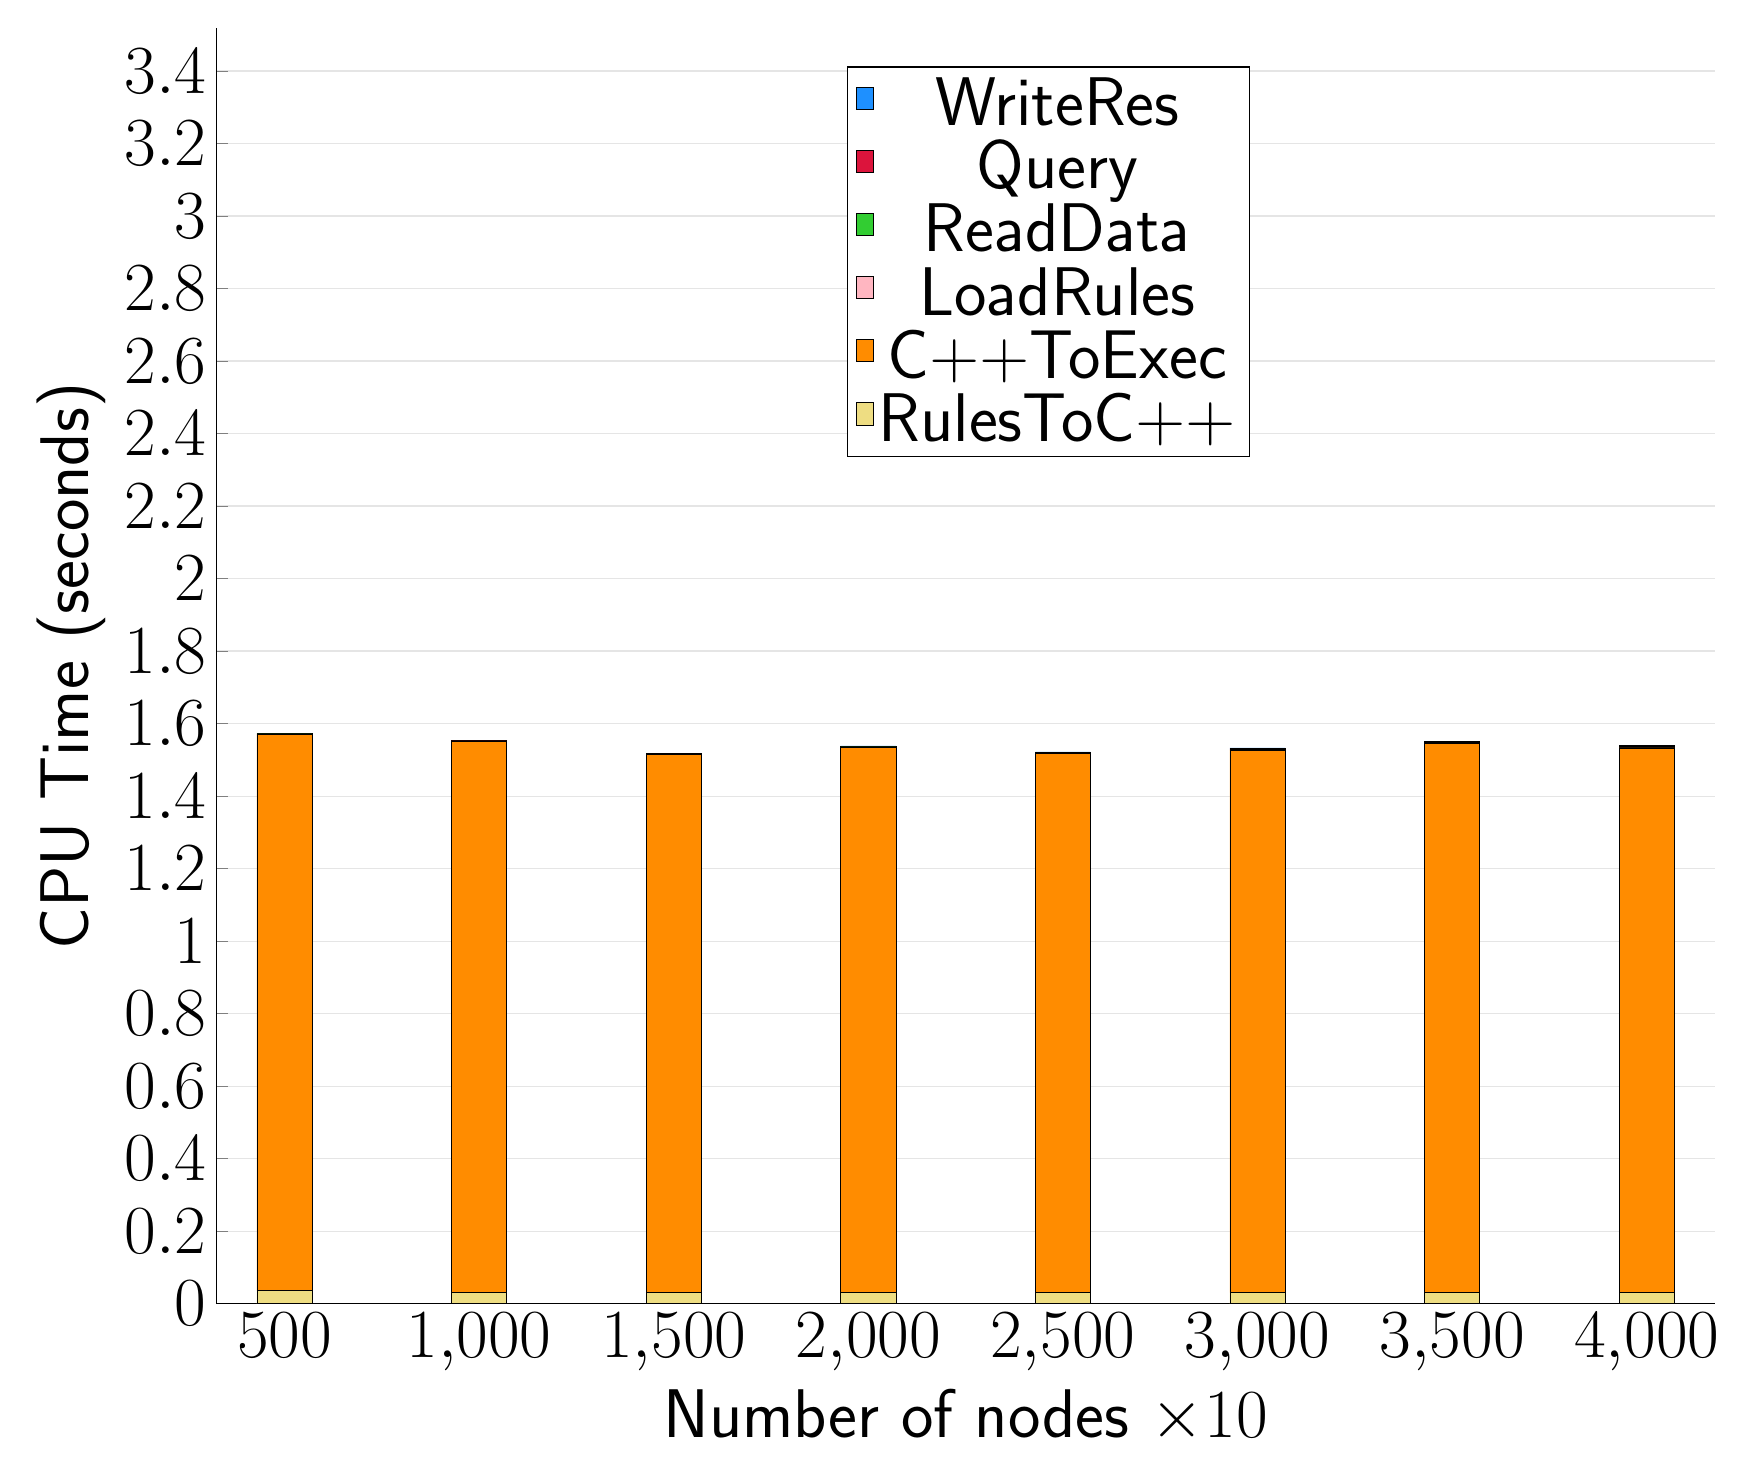
\begin{tikzpicture}
	\begin{axis}[
			ybar stacked,
			width=1.7\textwidth,
			bar width=0.7cm,
			ymajorgrids, tick align=inside,
			major grid style={draw=gray!20},
			xtick=data,
			ymin=0, ymax=3.518,
			axis x line*=bottom,
			axis y line*=left,
			enlarge x limits=0.05,
			legend style={
					at={(0.69, 0.97)},
					anchor=north east,
					legend columns=1,
					font=\Huge,
				},
			ylabel={CPU Time (seconds)},
			xlabel={Number of nodes $\times 10$},
			label style={font=\Huge},
			tick label style={font=\Huge},
		]
		\addlegendimage{fill=DodgerBlue, draw=black, line width=0.2pt}
		\addlegendentry{WriteRes}
		\addlegendimage{fill=Crimson, draw=black, line width=0.2pt}
		\addlegendentry{Query}
		\addlegendimage{fill=LimeGreen, draw=black, line width=0.2pt}
		\addlegendentry{ReadData}
		\addlegendimage{fill=LightPink, draw=black, line width=0.2pt}
		\addlegendentry{LoadRules}
		\addlegendimage{fill=DarkOrange, draw=black, line width=0.2pt}
		\addlegendentry{C++ToExec}
		\addlegendimage{fill=LightGoldenrod, draw=black, line width=0.2pt}
		\addlegendentry{RulesToC++}
		\addplot +[fill=LightGoldenrod, draw=black, line width=0.2pt] coordinates {
				(500, 0.036)
				(1000, 0.031000000000000007)
				(1500, 0.030000000000000006)
				(2000, 0.031000000000000007)
				(2500, 0.030000000000000006)
				(3000, 0.030000000000000006)
				(3500, 0.030000000000000006)
				(4000, 0.030000000000000006)
			};
		\addplot +[fill=DarkOrange, draw=black, line width=0.2pt] coordinates {
				(500, 1.535)
				(1000, 1.52)
				(1500, 1.485)
				(2000, 1.504)
				(2500, 1.487)
				(3000, 1.4969999999999999)
				(3500, 1.5160000000000002)
				(4000, 1.503)
			};
		\addplot +[fill=LightPink, draw=black, line width=0.2pt] coordinates {
				(500, 1.6100000000000002e-05)
				(1000, 0.0)
				(1500, 0.0)
				(2000, 1e-05)
				(2500, 0.0)
				(3000, 0.0)
				(3500, 0.0)
				(4000, 0.0)
			};
		\addplot +[fill=LimeGreen, draw=black, line width=0.2pt] coordinates {
				(500, 0.0004419)
				(1000, 0.0004555999999999999)
				(1500, 0.0006709000000000001)
				(2000, 0.0006914)
				(2500, 0.0008541)
				(3000, 0.0009691999999999999)
				(3500, 0.0009981)
				(4000, 0.0010842)
			};
		\addplot +[fill=Crimson, draw=black, line width=0.2pt] coordinates {
				(500, 0.0004941)
				(1000, 0.0007919000000000001)
				(1500, 0.0014496)
				(2000, 0.0017690999999999998)
				(2500, 0.0023275000000000006)
				(3000, 0.0029155000000000006)
				(3500, 0.0030510000000000003)
				(4000, 0.0034281)
			};
		\addplot +[fill=DodgerBlue, draw=black, line width=0.2pt] coordinates {
				(500, 0.0004798)
				(1000, 0.0006351)
				(1500, 0.0009605000000000001)
				(2000, 0.0011011)
				(2500, 0.0014053)
				(3000, 0.0017162)
				(3500, 0.0017322999999999998)
				(4000, 0.0019574)
			};
	\end{axis}
\end{tikzpicture}

\end{document}
